\documentclass[a4paper,11pt]{article}

\usepackage[utf8]{inputenc} % Unicode support (Umlauts etc.)
\usepackage[ngerman]{babel} % Change hyphenation rules
\usepackage{ziffer} % , können in Zahlen verwendet werden ohne Formatierung kaputt zu machen
\usepackage[top=25mm,right=25mm,bottom=20mm,left=25mm,includefoot]{geometry} % Seitenränder

\usepackage[fleqn]{amsmath} % Formatierte Gleichungen
\usepackage{graphicx} % Grafiken
\usepackage{xcolor} % Farbe in Text
\usepackage{fancyhdr} % Seitenstil mit Kopfzeile etc.

\usepackage{cases} % FAllunterscheidungen mathematisch uebereinander

\pagestyle{fancy}
\fancyhf{}
\lhead{Lösung Übungsblatt 4}
\rhead{Sascha Majewsky / Nils Hodys}
\rfoot{Seite \thepage}

\setlength{\parindent}{0cm} % Keine Einrückung der 1. Zeile eines Absatzes

\begin{document}
\section*{Aufgabe 1}

\subsection*{Entscheidungsvariablen}
\begin{flushleft}
    Kontinuierliche Variablen: \\
    $x_{s}$: Zu produzierender Schnaps in Hektar Ackerfläche pro Anbauperiode \\
    $x_{b}$: Zu produzierendes Bier in Hektar Ackerfläche pro Anbauperiode \\
    $x_{w}$: Zu produzierender Wein in Hektar Ackerfläche pro Anbauperiode \\
    \bigbreak
    Binärvariablen: \\
    \begin{numcases}{ys=}
        1, & wenn Schnapsproduktion mit Fixkosten 3900 GE \\
        0, & sonst keine Schnapsproduktion mit keinen Fixkosten
    \end{numcases}
    \begin{numcases}{yb=}
        1, & wenn Bierproduktion mit Fixkosten 4900 GE \\
        0, & sonst keine Bierproduktion mit keinen Fixkosten
    \end{numcases}
    \begin{numcases}{yw=}
        1, & wenn Weinproduktion mit Fixkosten 6600 GE \\
        0, & sonst keine Weinproduktion mit keinen Fixkosten
    \end{numcases}
    % example complex numcase
    %\begin{numcases}
        %{Opt\left(P, i, \ell \right)=min }
         %(1)\hspace{0.5 mm} Opt(P,i+1,\ell) + M(\ell,g)\label{eq:1}\hspace*{-10em} & \nonumber\\ % Put the command \nonumber before \\ and do not put \\ after the last line in order not to create a new equation line.
         %(2)\hspace{0.5 mm} \min_{g \in L(v_{i+1})}\{Opt(P,i+1,g) + M(\ell,g)\}\label{eq:2}\hspace*{-5em} & \nonumber
    %\end{numcases}
\end{flushleft}

\subsection*{Modellierung}
\begin{flushleft}
    Anmerkung: \\
    - Es gibt keine Mindestbestellmengen an Ackerfläche pro Jahr pro Produkt und daher sind in Bezug dessen keine Schwellenwerte zu beachten \\
    \bigbreak
    Zielfunktion: \\
    - Zielfunktion mit Maximierungsausrichtung abzüglich Fixkosten
\end{flushleft}

\begin{align*}
    \text{max. } & z = 15000x_{s} + 27000x_{b} + 36000x_{w} - 3900y_{s} - 4900y_{b} - 6600y_{w} \\
    \\
    \text{s.t. } & x_{s} + x_{b} + x_{w} \le 100 && \text{Max. Gesamtanbaufläche 100 Hektar} \\
    & 60x_{s} + 60x_{b} + 48x_{w} \le 5200 && \text{Erträge pro Hektar in 50 Liter Fass} \\
    & x_{s} \le 60*y_{s} && \text{Schnaps Höchstproduktion u. Binärverknüpfung} \\
    & x_{b} \le 50*y_{b} && \text{Bier Höchstproduktion u. Binärverknüpfung} \\
    & 2400x_{w} \le 145000*y_{w} && \text{Wein Höchstproduktion u. Binärverknüpfung} \\
    & x_{s}, x_{b}, x_{w} \ge 0 && \text{Es kann keine negative Menge produziert werden} \\
    & y_{s}, y_{b}, y_{w} \in \{ 0,1 \} && \text{Wertzuweisung Binärvariablen} \\
\end{align*}

\subsection*{Lingo Solver}
\begin{centering}
	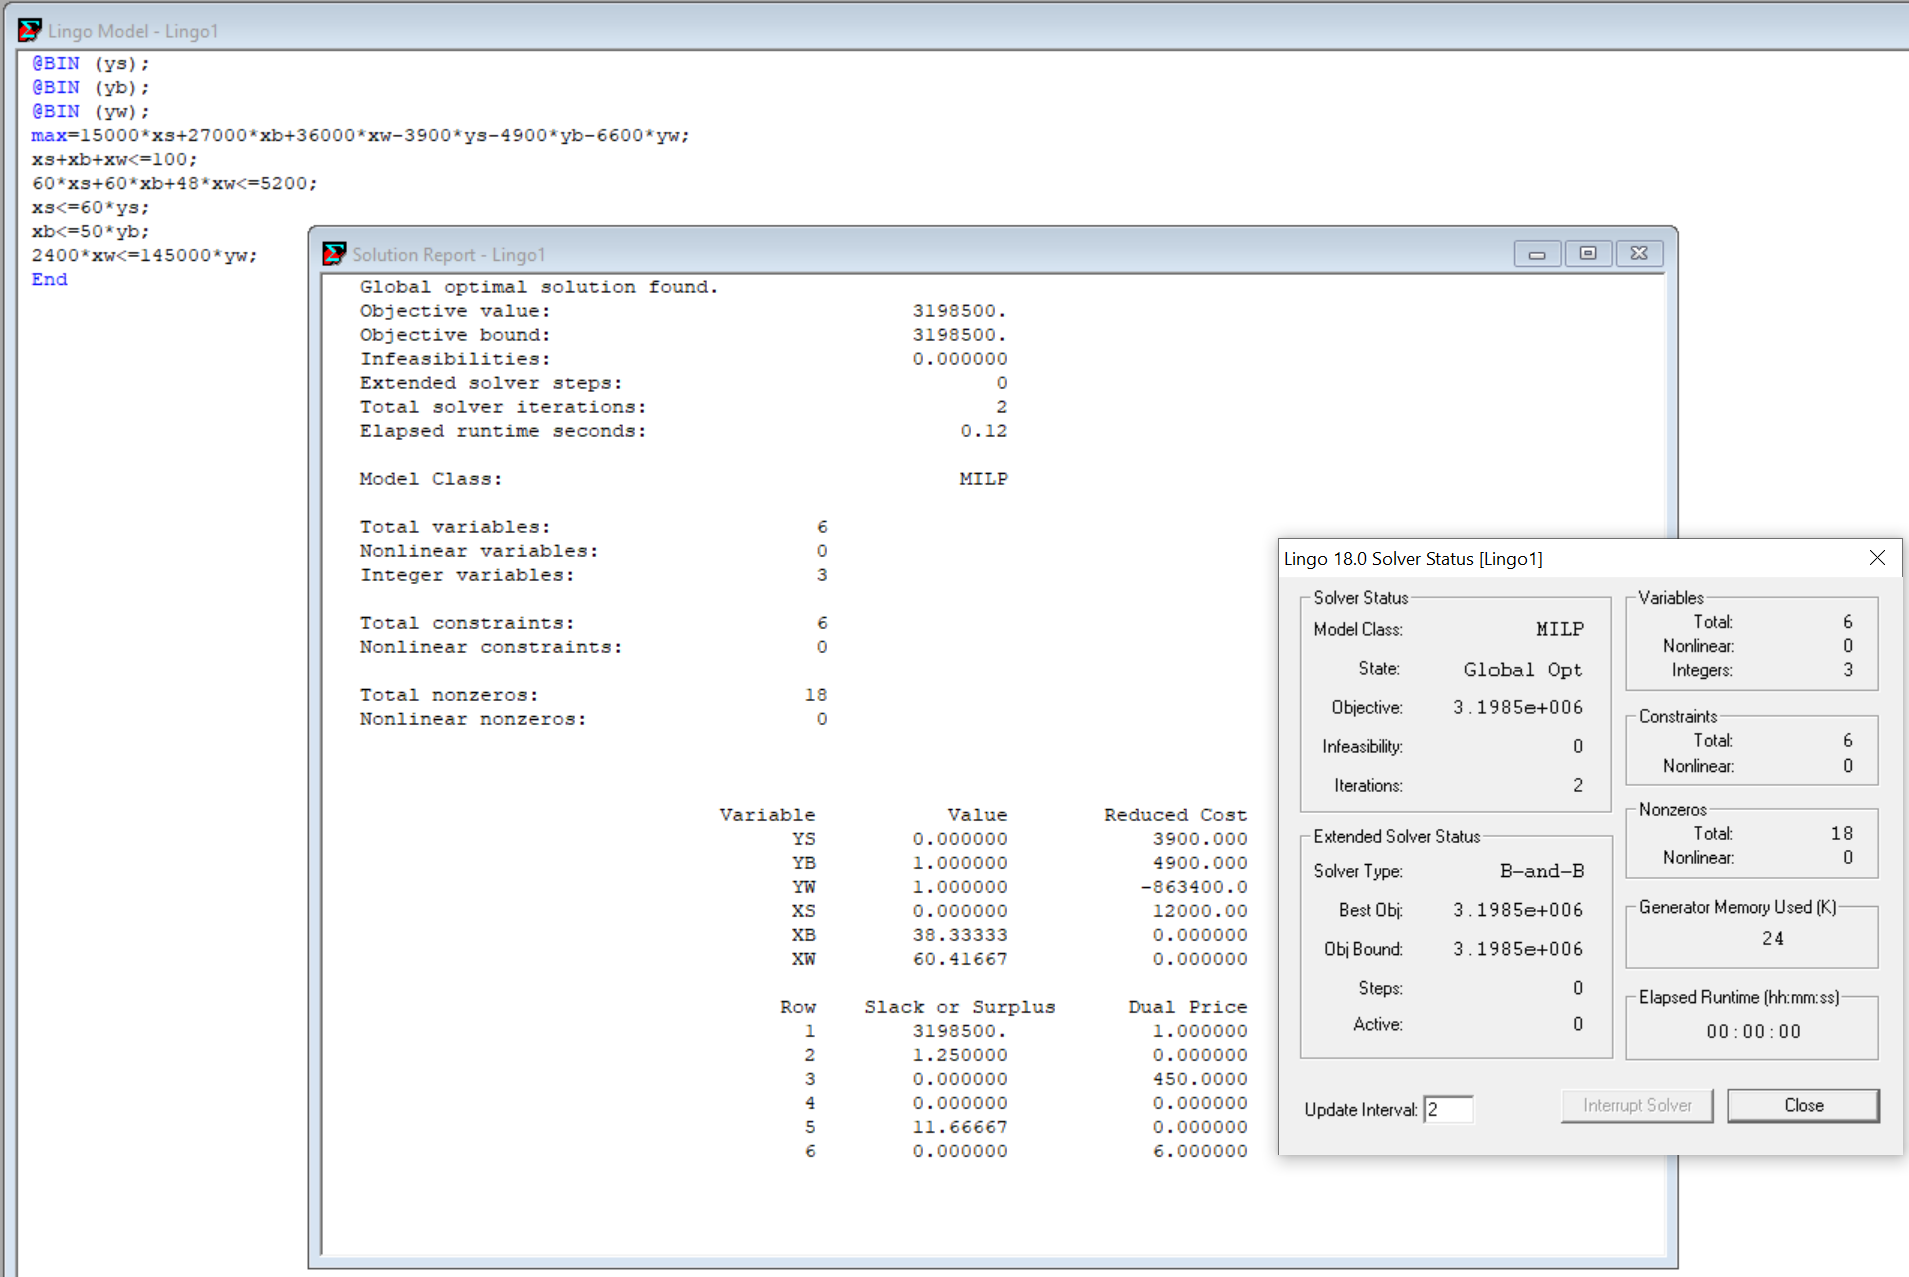
\includegraphics[width=1\linewidth]{src/blatt_4_aufgabe_1_loesung_solver.PNG}
\end{centering}

$\to$ \textbf{Getränkeherstellerberatung Optimalfall:} \\
- Im Optimalfall wird pro Anbauperiode nur Bier und Wein angebaut \\
- Dann verteilt sich die Bestellung des Ackers pro Anbauperiode auf 38,33333 ha Hopfen und 60,41667 ha Weintrauben \\
- Es bleiben auf Grund der Restriktionen der Abfülling in 50l Fässer pro Anbauperiode 1,25 ha nutzbarer Ackerfläche übrig, welche privat oder für andere wirtschaftliche Geschäfte genutzt werden kann

\section*{Aufgabe 2}

\subsection*{Entscheidungsvariablen}
\begin{flushleft}
    Kontinuierliche Variablen: \\
    $x_{m}$: Anzurichtender Salat M in Portionen \\
    $x_{l}$: Anzurichtender Salat L in Portionen \\
    $x_{c}$: Anzurichtender Salat C in Portionen \\
    \pagebreak
    Binärvariablen: \\
    \begin{numcases}{ym=}
        1, & wenn Anrichtung Salat M mindestens 30 Portionen \\
        0, & sonst keine Anrichtung Salat M
    \end{numcases}
    \begin{numcases}{yl=}
        1, & wenn Anrichtung Salat L mindestens 30 Portionen \\
        0, & sonst keine Anrichtung Salat L
    \end{numcases}
    \begin{numcases}{yc=}
        1, & wenn Anrichtung Salat C mindestens 30 Portionen \\
        0, & sonst keine Anrichtung Salat C
    \end{numcases}
\end{flushleft}

\subsection*{Modellierung}
\begin{flushleft}
    Anmerkung: \\
    - Falls ein Salat angerichtet wird gibt es eine Mindestmenge (30), daher werden Schwellenwerte relevant \\
    - Ein Schwellenwert ist entweder 0 oder Mindestmenge bis Höchstmenge \\
    - Uns ist die Mindestmenge mit 30 Portionen bekannt, daher ist eine Ermittlung mittels Big-M durch Restriktionsbeziehungen nicht nötig
    \bigbreak
    Zielfunktion: \\
    - Zielfunktion mit Maximierungsausrichtung und Binärverknüpfung
\end{flushleft}

%\subsection*{LP}
\begin{align*}
    \text{max. } & z = 3,90x_{m} * y_{m} + 4,30x_{l} * y_{l} + 3,60x_{c} * y_{c} \\
    \\
    \text{s.t. } & x_{m} + x_{l} + x_{c} \le 180 && \text{6 Mitarbeiter können täglich 30 Salate anrichten} \\
    & 300x_{m} + 200x_{l} + 250x_{c} \le 48000 && \text{Tomatenbestand Gramm} \\
    & 150x_{m} + 110x_{l} + 150x_{c} \le 25000 && \text{Paprikabestand Gramm} \\
    & 150x_{m} + 120x_{c} \le 19000 && \text{Gurkenbestand Gramm} \\
    & 200x_{l} \le 11000 && \text{Mangobestand Gramm} \\
    & 250x_{m} \le 8000 && \text{Rucolabestand Gramm} \\
    & 180x_{l} \le 6000 && \text{Avocadobestand Gramm} \\
    & 220x_{c} \le 12000 && \text{Kichererbsenbestand Gramm} \\
    & 40x_{m} + 35x_{l} \le 5000 && \text{Olivenölbestand Gramm} \\
    & 70x_{c} \le 5000 && \text{Fetabestand Gramm} \\
    & x_{m} \ge 30*y_{m} && \text{Salat M Binärverknüpfung} \\
    & x_{l} \ge 30*y_{l} && \text{Salat L Binärverknüpfung} \\
    & x_{c} \ge 30*y_{c} && \text{Salat C Binärverknüpfung} \\
    & x_{m}, x_{l}, x_{c} \ge 0 && \text{Es kann keine negative Menge angerichtet werden} \\
    & y_{m}, y_{l}, y_{c} \in \{ 0,1 \} && \text{Wertzuweisung Binärvariablen} \\
\end{align*}

\subsection*{Lösung laut Solver}
\begin{centering}
	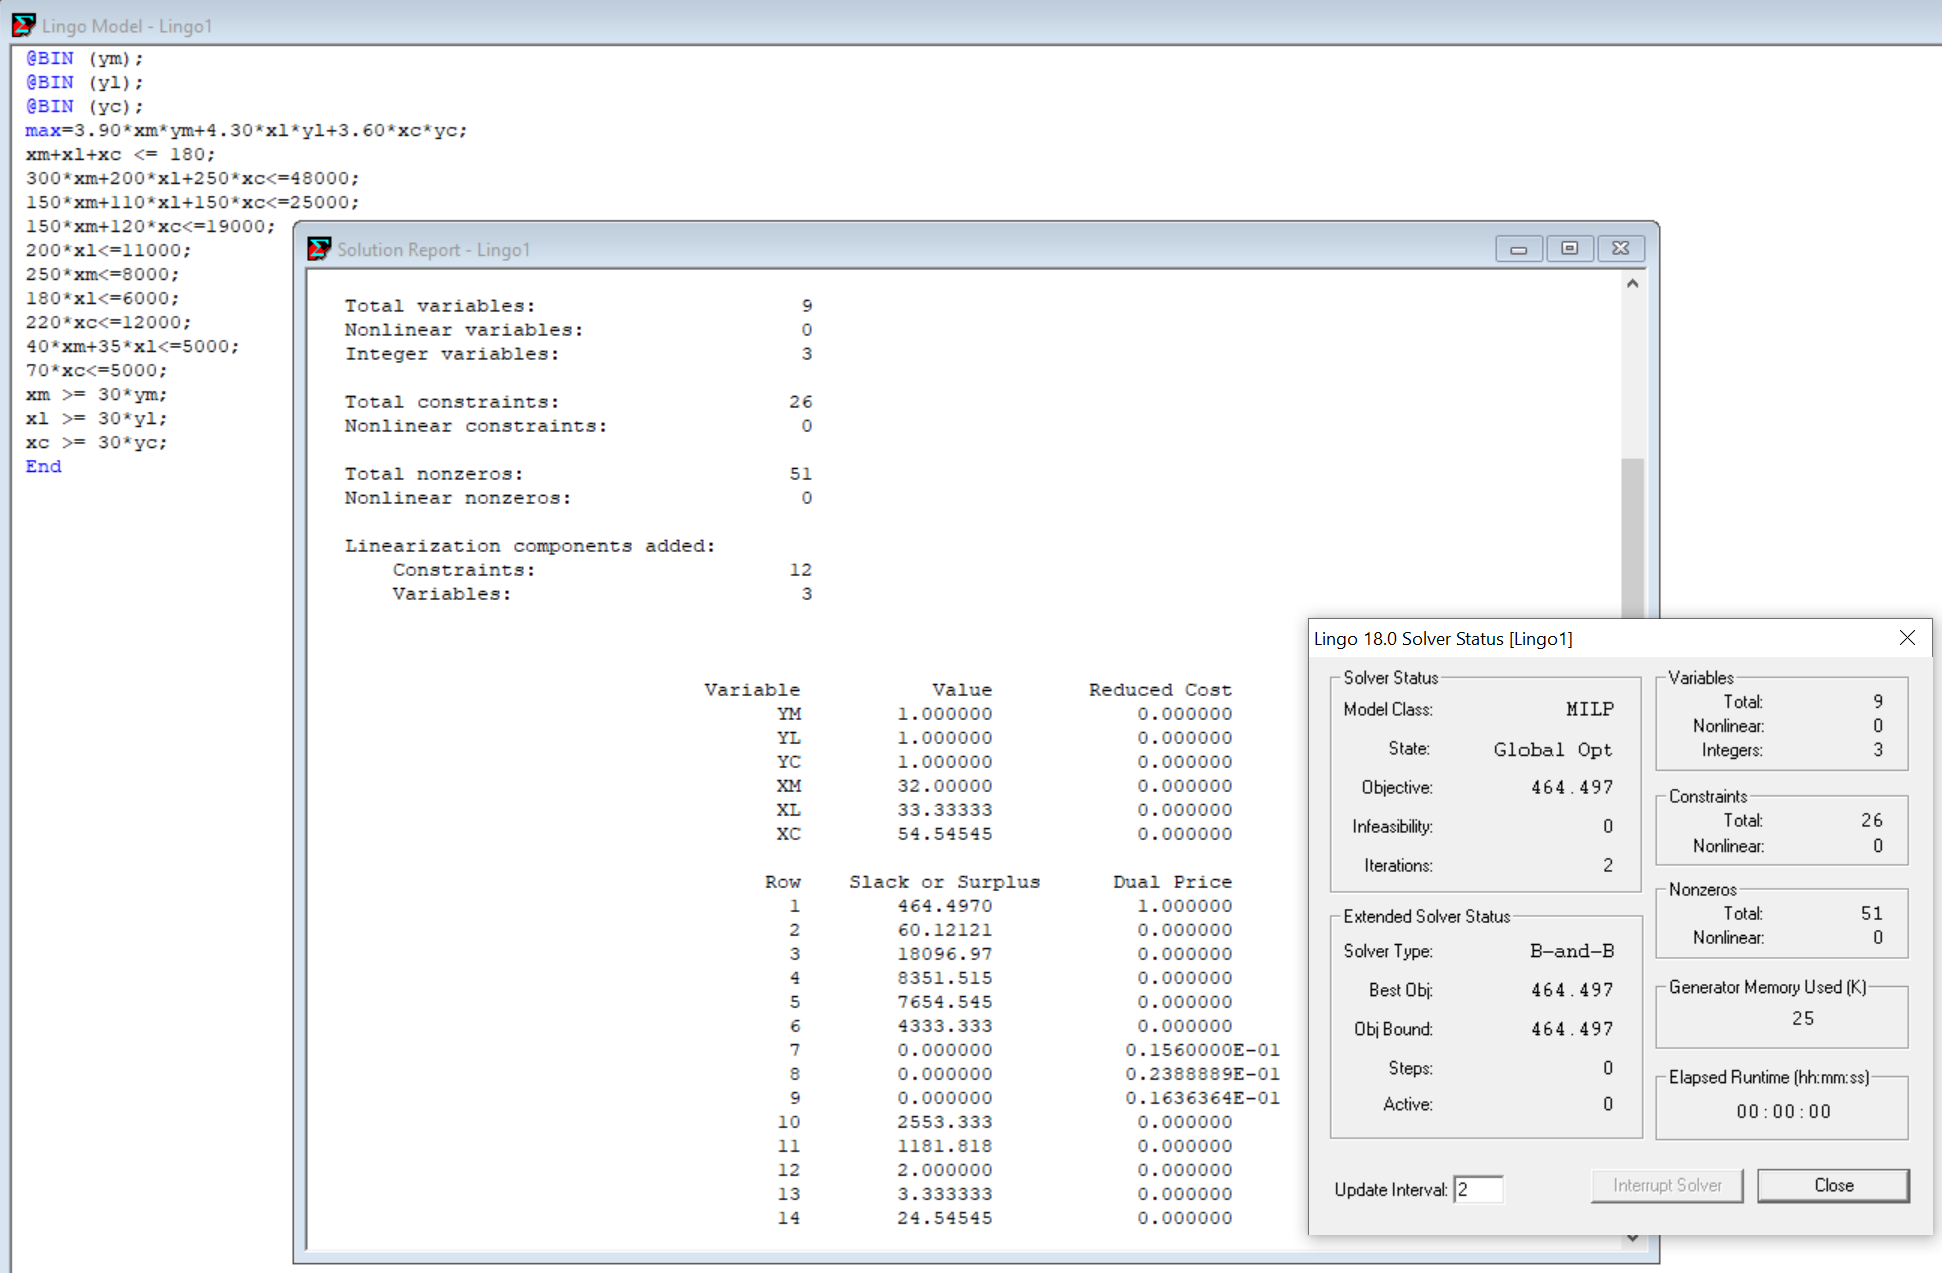
\includegraphics[width=1\linewidth]{src/blatt_4_aufgabe_2_loesung_solver.PNG}
\end{centering}

$\to$ \textbf{Salatbar Optimalfall:} \\
- Jede Salatart wird angerichtet \\
- Salat M wird in 32 Portionen, Salat L in 33 Portionen und Salat C in 54 Portionen produziert

\end{document}